\chapter{Identifying contribution activities in a ``code-centric" community}
\chaptermark{Contribution activities}
\label{identifyng-contribution:chapter}

While contributions to the digital commons of FLOSS communities, such as source code and documentation, have been widely explored, other types of contribution have remained less visible. In order to address how the Drupal community self-organises by exploring contribution activities, it was necessary to first study what kinds of activities are perceived as contribution by Drupalistas.

This chapter provides empirical evidence of the perception of ``community-oriented" activities as contributions, their lack of visibility in digital collaboration platforms, and their relevance for the sustainability of the community. Additionally, the chapter connects this issue to the larger literature on the commons, by drawing on the concept of affective labour.

\section{Contribution beyond source code in FLOSS}

The notion of contribution is central to the understanding of the phenomenon of FLOSS, as well as in CBPP in general. As argued by \textcite{wittel2013counter}, CBPP communities focussed on the production of digital commons, such as in the case of FLOSS, typically possess an economy of contribution, meaning they are not based on direct reciprocity. This contrasts with an economy of gift, which is based on direct reciprocity. For example, in the specific case of FLOSS the concept of contribution has been widely employed in studies, but mainly in reference to activities related to source code. This can be understood as part of the ``code-centric" character --- considering source code the most valuable type of contribution --- of FLOSS communities, which has been reflected in the research on FLOSS.

For example, the \citeauthor{VonKrogh2006}'s (\citeyear{VonKrogh2006}) literature review on FLOSS discussed in section \ref{subsubsec:state-art:floss:academic-research} shows how studies that include the notion of contribution have principally examined the development of source code as the main type of contribution. This can be observed, for example, in studies focussed on motivations to contribute \parencite[e.g.,][]{bergquist2001power,  ghosh2002free, Lerner2002, dalle2003allocation, lakhani2003hackers, stenborg2004explaining}; as well as in those focussed on the relationship between organisation and contribution \parencite[e.g.,][]{franck2002reconciling, dempsey2002open, koch2002effort, grewal2006location, maccormack2006exploring}.

Another illustration of this ``code-centrism" in research on FLOSS can be found in the literature review of \textcite{crowston2012free}, in which they developed a framework based on an inputs-mediators-outputs-inputs model\footnote{This refers to an extension of the earlier Input-Process-Output model \parencite{hackman1975group} that, among other differences, distinguishes emergent states from processes. \textcite{crowston2012free} applied the inputs-mediators-outputs-inputs model characterising, for example, FLOSS community members' characteristics as inputs, decision-making as processes, roles as emergent states, and team performance as outputs.} \parencite{ilgen2005teams} to review 135 papers. In the case of inputs, most of the literature related to individual participation considers source code related activities \parencite[e.g.,][]{luthiger2005fun, robles2005evolution, Roberts2006, fershtman2007open}. A similar ``code-centric" character can be observed with regard to the outputs, for example regarding FLOSS team performance \parencite[e.g.,][]{bezroukov1999second, samoladas2004open, gyimothy2005empirical, de2005handling}. A few studies on the level of commitment have moved the focus from code contribution \parencite[e.g.,][]{mockus2000case, mockus2002two} to explore communication contributions \parencite{crowston2006hierarchy} and support contributions \parencite{lakhani2003open}.

This study continues this shift. Firstly, this study aims to widen the notion of contribution using a social constructivist perspective, in which contribution in FLOSS and CBPP communities can be understood as a \textsl{set of meanings which are constantly evolving through negotiation among the community members.} Secondly, it unveils the outcomes from contributions which have remained less visible, including those that are intangible, such as excitement, kinship, passion, familiarity, reciprocity, or sense of community, all of which have been identified as participation motivators in FLOSS communities \parencite[e.g.,][]{zeitlyn2003gift, freeman2007material, fang2009understanding}. To this end, this study draws on \citeauthor{hardt1999affective}'s (\citeyear{hardt1999affective}) concept of affective labour, defined as the immaterial labour present in human interaction that creates or modifies emotional experiences.

The relevance of affective labour in CBPP communities is of increasing interest to CBPP scholars. \textcite{Bollier2014} cited the study of \textcite{Singh2013} on the importance of affective labour in CBPP communities, labelling affective labour as its ``lifeblood". \textcite{Singh2013} provides a compelling case study of the dynamics of affective labour in the non-digital domain, by examining the daily practices of a community-based initiative to protect and regenerate a forest in Odisha (India). In the context of environmental politics, Singh explored how the participants of this community-based initiative became conservationists, arguing that the efforts carried out by these participants entailed affective labour, transforming not only the object, the forest in this particular case, but also the individual and collective subjectivities of the participants. This thesis explores a similar set of dynamics occurring in CBPP communities, looking at the Drupal community as a case study, exploring how certain contribution activities transform participants' subjectivities so that they become ``Drupalistas".

The study of which activities are considered contributions by a community's members becomes especially relevant in an extreme case such as the Drupal community, whose prominent ``code-centric" facet has been shown in previous literature \parencite{Zilouchian2011, Sims2013}. This ``code-centrism" is illustrated by the well-known Drupal motto: ``Talk is silver, code is gold\footnote{As illustrative examples, the motto can be found in relevant Drupal blogs such as that of the Drupal Association (see \url{https://assoc.drupal.org/node/709}, accessed on \nth{25} July 2015), or the official blog of the largest Drupal business company, Acquia (see \url{http://www.acquia.com/blog/talk-silver-code-gold-acquias-code-contributions-drupal-project}, accessed on \nth{25} July 2015).}". The motto embodies the traditional belief in FLOSS communities that the most valuable type of contribution that a participant can provide is source code.

With this goal in mind, qualitative research was undertaken to highlight activities not widely studied due to their traditional lack of visibility in comparison with activities ``officially" considered contributions (e.g. those listed in the main collaboration platform\footnote{See \url{https://www.drupal.org/contribute}, accessed on \nth{30} April 2014.}). It is argued that these less visible activities enable the creation of individual and collective subjectivities among members of the Drupal community, and are a significant factor in its sustainability.

\section{``Object-oriented" and ``community-oriented" contribution activities}
\label{subsec:insights:contrib-beyond-source-code}

When studying what types of activities are perceived as contributions in the Drupal community, two main types of contribution activities emerged. The first was ``object-oriented" contributions, encompassing all the activities whose focus of action are objects, typically digital commons such as source code, documentation and translations. The second category is ``community-oriented" contributions: those in which the focus of action is directed towards the community. Examples are the organisation and participation in face-to-face events, activities related to supporting other users, and mentoring. Table \ref{contributions-list} provides a summary of the contribution activities identified in this study. The categories are based on the analysis of all the data collected for the first thematic area --- notion of contribution --- presented in section \ref{sec:data-collection}.


%%% BEGIN CONTRIBUTIONS TABLE
%%%%%%%%%%%%%%%%%%%

    \scriptsize

    \setlength\LTleft{0pt}
    \setlength\LTright{0pt}

\begin{longtable}[c]{|p{0.2\textwidth}|p{0.25\textwidth}|p{0.22\textwidth}|p{0.15\textwidth}}

    \hline
    \multirow{20}{1in}{``Object-oriented" (G\textunderscript{1})} & \multirow{11}{1in}{Source code (SG\textunderscript{1.1})}                                  & \multirow{6}{1in}{\textit{Core} projects (SG\textunderscript{1.1.1})} & \multicolumn{1}{p{0.25\textwidth}|}{Lead development initiatives} \\ \cline{4-4}
    & & & \multicolumn{1}{p{0.25\textwidth}|}{Participate in development initiatives} \\ \cline{4-4}
    & & & \multicolumn{1}{p{0.25\textwidth}|}{Submission of patches} \\ \cline{4-4}
    & & & \multicolumn{1}{p{0.25\textwidth}|}{Review and test patches} \\ \cline{4-4}
    & & & \multicolumn{1}{p{0.25\textwidth}|}{Summarise issues} \\ \cline{4-4}
    & & & \multicolumn{1}{p{0.25\textwidth}|}{Report bugs} \\ \cline{3-4}
    & & \multirow{4}{1in}{\textit{Contributed} projects (SG\textunderscript{1.1.2})} & \multicolumn{1}{p{0.25\textwidth}|}{Maintain project (e.g. review of patches, port to new version, add new features, etc.)}             \\ \cline{4-4}
    & & & \multicolumn{1}{p{0.25\textwidth}|}{Submit patches} \\ \cline{4-4}
    & & & \multicolumn{1}{p{0.25\textwidth}|}{Review new applications} \\ \cline{4-4}
    & & & \multicolumn{1}{p{0.25\textwidth}|}{Report bugs} \\ \cline{3-4}
    & & Share other \textit{custom} projects --- with a FLOSS license, but out of Drupal.org (SG\textunderscript{1.1.3}) & \\ \cline{2-3}
    & \multirow{3}{1in}{Documentation at Drupal.org (SG1.2)}                   & Write documentation & \\ \cline{3-3}
    & & Moderate documentation & \\ \cline{3-3}
    & & Report issues with documentation (e.g. spam) & \\ \cline{2-3}
    & \multirow{3}{1in}{Translation (SG\textunderscript{1.3})}                                   & Provide translation strings & \\ \cline{3-3}
    & & Review/approve translation strings & \\ \cline{3-3}
    & & Translation group management & \\ \cline{2-3}
    & \multirow{3}{1in}{Design (SG\textunderscript{1.4})} & User interface design & \\ \cline{3-3}
    & & User experience & \\ \cline{3-3}
    & & Design of logos, style guides, etc. & \\ \cline{1-3}
    \multirow{35}{1in}{``Community-oriented" (G\textunderscript{2})} & \multirow{3}{1in}{Usage and support (SG\textunderscript{2.1})}                             & Provide specific support to other users through the official platform (e.g. forums, IRC, etc.) & \\ \cline{3-3}
    & & Provide specific support to others through other platforms (e.g. drupal.stackexchange.com) & \\ \cline{3-3}
    & & Provide generic advises (e.g. ``recipees" about how to build certain functionality, experience with certain modules, etc.) & \\ \cline{2-3}
    & \multirow{4}{1in}{Evangelisation (SG\textunderscript{2.2})}                                & Create Drupal related materials (e.g. blog posts, videos, podcasts, etc.) & \\ \cline{3-3}
    & & ``Spread the word" of Drupal on a day-to-day basis (e.g. talk about Drupal with colleagues,promote Drupal in FLOSS conferences, etc.) & \\ \cline{3-3}
    & & Create initiatives around the Drupal ecosystem (e.g. Drupical.com, Drupalfund.us, etc.) & \\ \cline{3-3}
    & & Marketing research and branding & \\ \cline{2-3}
    & \multirow{2}{1in}{Training and mentoring (SG\textunderscript{2.3})}                        & Creation of training materials (e.g.: drupallader.org) & \\ \cline{3-3}
    & & Mentoring contributors (e.g. Core mentoring, students from Google Summer of Code, etc.) & \\ \cline{2-3}
    & \multirow{4}{1in}{Online community management (SG\textunderscript{2.4})}                   & Participation in Drupal.org Content Working Group (e.g. curation, moderation, etc.) & \\ \cline{3-3}
    & & Participation in Drupal.org software Working Group (e.g.: tasks related to the maintenance of the software run at the main platform of collaboration) & \\ \cline{3-3}
    & & Participation in Drupal.org. infrastructure Working Group (e.g. tasks related to server administration) & \\ \cline{3-3}
    & & Participation in groups.drupal.org (e.g. local groups,legal support, conflict resolution, etc.) & \\ \cline{2-4}
    & \multirow{18}{1in}{Organisation and participation in F2F events (SG\textunderscript{2.5})} & \multirow{3}{1in}{Local events (SG\textunderscript{2.5.1})} & \multicolumn{1}{p{0.25\textwidth}|}{Organisation of the event (e.g. logistics)} \\ \cline{4-4}
    & & & \multicolumn{1}{p{0.25\textwidth}|}{Give talks, run workshops, etc} \\ \cline{4-4}
    & & & \multicolumn{1}{p{0.25\textwidth}|}{Attendance at the event} \\ \cline{3-4}
    & & \multirow{5}{1in}{\textit{DrupalCamps} / Drupal Dev Days / Frontend United and other regional or role-specific events (SG\textunderscript{2.5.2})} & \multicolumn{1}{p{0.25\textwidth}|}{Organisation of the event (e.g. logistics, selection of presentations, etc.)}                       \\ \cline{4-4}
    & & & \multicolumn{1}{p{0.25\textwidth}|}{Creation of the website, social media management, etc.}                                             \\ \cline{4-4}
    & & & \multicolumn{1}{p{0.25\textwidth}|}{Prepare a presentation} \\ \cline{4-4}
    & & & \multicolumn{1}{p{0.25\textwidth}|}{Run a BoF (Birds Of a Feather)} \\ \cline{4-4}
    & & & \multicolumn{1}{p{0.25\textwidth}|}{Attendance at the event} \\ \cline{3-4}
    & & \multirow{10}{1in}{\textit{DrupalCon} (SG\textunderscript{2.5.3})} & \multicolumn{1}{p{0.25\textwidth}|}{Organisation of the event (e.g. logistics, selection of presentations, etc.)}                       \\ \cline{4-4}
    & & & \multicolumn{1}{p{0.25\textwidth}|}{Creation of the website, social media management, etc.}                                             \\ \cline{4-4}
    & & & \multicolumn{1}{p{0.25\textwidth}|}{Coordination of the local community with the Drupal Association}                                    \\ \cline{4-4}
    & & & \multicolumn{1}{p{0.25\textwidth}|}{Volunteering in the event (e.g. provide assistance to find rooms, registration desks, etc.)}        \\ \cline{4-4}
    & & & \multicolumn{1}{p{0.25\textwidth}|}{Prepare a presentation} \\ \cline{4-4}
    & & & \multicolumn{1}{p{0.25\textwidth}|}{Run a BoF} \\ \cline{4-4}
    & & & \multicolumn{1}{p{0.25\textwidth}|}{Participate in Code Sprints} \\ \cline{4-4}
    & & & \multicolumn{1}{p{0.25\textwidth}|}{Participate in Community Summit} \\ \cline{4-4}
    & & & \multicolumn{1}{p{0.25\textwidth}|}{Participate in ``Tour de Drupal"} \\ \cline{4-4}
    & & & \multicolumn{1}{p{0.25\textwidth}|}{Organisation of social events (e.g. Drupal Trivia night)} \\ \cline{2-4}
    & \multirow{4}{1in}{Economic sustainability (SG\textunderscript{2.6})}                       & Become a member of the Drupal Association & \\ \cline{3-3}
    & & Donation to the Drupal Association & \\ \cline{3-3}
    & & Donate to crowdfunding campaigns for \textit{core} or \textit{contrib} projects & \\ \cline{3-3}
    & & Sponsorship of F2F events & \\ \cline{1-3}

    \caption[List of identified types of contributions]{List of identified types of contributions.}
    \label{contributions-list}
    \end{longtable}

    \normalsize

    %%% END CONTRIBUTIONS TABLE
    %%%%%%%%%%%%%%%%%%%

The activities are firstly classified according to the main categories: ``object-oriented" (G\textunderscript{1}) and ``community-oriented" (G\textunderscript{2}). Contribution activities related to source code (SG\textunderscript{1.1}) are further classified into three subgroups: \textit{core} (SG\textunderscript{1.1.1}), \textit{contributed} (SG\textunderscript{1.1.2}) and FLOSS \textit{custom} projects (SG\textunderscript{1.1.3}) not included in Drupal.org. The reason for this distinction is the significant differences found in the organisational aspects of the socio-technical systems that surround these contribution activities, despite the type of object being the same: source code. For example, the possibility to perform modifications in the digital commons for the \textit{core} group is more formalised, typically harder to achieve, and more specialised. As a consequence, new contribution activities emerge and are valued as such. For example, the ``creation of summaries of the issues", in which hundreds of comments are summarised, is perceived as a valuable contribution. This type of contribution is typically carried out by newer members to save core developers having to read the whole list. It is encouraged as a way to ``contribute to core", whilst enabling the newest members to become familiar with the organisational processes and the technicalities.

In a similar way, within the ``community-oriented" group (G\textunderscript{2}), a distinction is made with regard to contribution activities related to the organisation and participation in face-to-face events (SG\textunderscript{2.5}). In this case, they are differentiated by their scope. The second of these subgroups (SG\textunderscript{2.5.2}) includes regional, national and role-specific events. This is because the dynamics, organisational processes and identified contribution activities in these events are similar. As in the case of the subgroup SG\textunderscript{1.1}, the main difference between SG\textunderscript{2.5.1}, SG\textunderscript{2.5.2} and SG\textunderscript{2.5.3} is with regard to the level of formalisation and the ease of participation in their organisation. For example, \textit{DrupalCon}  activities, largely organised by the most formal institution within the Drupal community, the Drupal Association, are at the formal end of the spectrum.

While, as previously discussed, ``object-oriented" activities have been widely employed in studies drawing on the notion of contribution, those whose main focus of action is the community have received less attention. This is despite the notion of community being central to understand CBPP, as suggested by a Drupalista who writes in his personal blog:

\begin{figure}[H]
    \centering
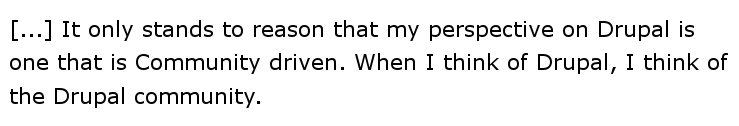
\includegraphics[scale=0.45]{img/quotes_replacement/quote_dougvann_com.png}
    \caption[Excerpt from the article ``Drupal is a community AND there happens to be a piece of software by the same name"]{Drupal developer, 6 years\protect\footnotemark . Excerpt from the article ``Drupal is a community AND there happens to be a piece of software by the same name". Retrieved \nth{20} September 2014, from \url{http://dougvann.com/blog/drupal-community-and-there-happens-be-piece-software-same-name}.}
    \label{quote_dougvann}
\end{figure}

\footnotetext{The attributes under the excerpts refer to the main role(s), gender and number of years of the Drupal.org accounts of the Drupalistas at the time the document was written or the interview was conducted.}

Similar views were also expressed during interviews, in which Drupalistas emphasised the community when asked about what was most important about Drupal and their involvement. For example, when asked about the meaning of Drupal, I\textunderscript{3} explained:

\begin{quotation}
    ``[...] it's [referring to Drupal] the community in which I spend most of my time. When I wake up, the first thing I do in the morning is check the Telegram group  which we are in [referring to an instant messaging group of Spanish Drupalistas], to see what people have been talking about. When I arrive at the office, the first thing that starts up is the IRC [Internet Relay Chat] client connecting to the Drupal channels."

\begin{flushright}\footnotesize{Drupal developer, M, 7 years. Original reply in Spanish.}\end{flushright}
\end{quotation}

These ``community-oriented" activities are indeed understood as contribution by Drupalistas. A comment from I\textunderscript{3} illustrates, for example, the relevance of activities such as the participation in and organisation of local face-to-face events for the health of the community:

\begin{quotation}
    ``[...] organising talks, meetups or just hanging out with Drupalistas to drink some beers and have a talk, are also very important activities, and very positive for the community."

\begin{flushright}\footnotesize{Drupal developer, M, 7 years. Original reply in Spanish.}\end{flushright}
\end{quotation}

Similarly, the following excerpt from field notes illustrates how some Drupalistas identify the participation in and organisation of offline events as contributions, as well as acknowledging differences with respect to the internal logics of value when compared to ``object-oriented" activities, such as contributing source code:

\begin{quotation}
    ``[..] She explained to me that we, as a community, are not aware sometimes of the relevance that other activities have, such as the organisation of events like this one [referring to the DrupalCamp] or the `Tour de Drupal\footnote{\label{footnote-drupal} ``Tour de Drupal" (\url{http://tourdedrupal.org/}) is an initiative of Drupalistas to cycle together during several days to the city in which the \textit{DrupalCon} is held. It was organised for the first time for \textit{DrupalCon} Europe 2014, when people cycled from several European cities to Amsterdam (\url{http://vimeo.com/107816807}).}'. She thought that organising and attending events like this one are definitely types of contribution, but they aren't so popular. She explained to me that we tend to think a lot in contributing code, especially to core, but she highlighted: `thanks to things like this [referring to the F2F event], the community is very healthy'."

\begin{flushright}\footnotesize{Extracted from full field notes during the participant observation at \textit{DrupalCamp} North East 2014.}\end{flushright}
    \end{quotation}

These perceptions of what can be considered contribution contrast with those represented in the main collaboration platform. Not surprisingly for a FLOSS community with a strong ``code-centric" character \parencite{Zilouchian2011, Sims2013}, there is a mismatch between the perceptions of the importance of ``community-oriented" activities and those ``officially" reflected in the main collaboration platform. This mismatch is illustrated, for example, in the main pages that explain how individuals could contribute to Drupal.

On the one hand, all the categories identified as ``object-oriented" (G\textunderscript{1}) are represented in the ``Get Involved" page\footnote{\url{https://drupal.org/contribute}, accessed on \nth{11} November 2014.} relating to contribution in the main collaboration platform.  Some of them are differentiated and highlighted. For example, in the case of contribution activities related to source code (SG\textunderscript{1.1}), there is an explicit distinction between `theming' and `backend' development.

On the other hand, ``community-oriented" activities (G\textunderscript{2})  are only partially reflected in user support, donations and marketing. For example, a sub-page named ``Contribute to Drupal.org\footnote{\url{https://drupal.org/contribute/drupalorg}, accessed on \nth{11} November 2014.}", provides information about contributions related to the main collaboration platform itself. This area refers to some of the ``online community management" (SG\textunderscript{2.4}) contributions. However, no explicit mention is made of the ``organisation and participation in face-to-face events" (SG\textunderscript{2.5}). The first reference can be found only after navigating through a secondary link in the ``General Resources" section to the Drupal Groups\footnote{\url{https://groups.drupal.org/}, accessed on \nth{11} November 2014.}. This allows the user to start browsing by geographical criteria after several steps, where the first references to the organisation of events can be found.

The main aim in this section has been to show the need to widen our understanding of contribution activities beyond the traditional view of source code or other ``object-oriented" activities, and the existence of differences with regard to the internal perceived value. Additionally, evidence was provided with regards to  the lack of visibility of  ``community-oriented" activities in the main collaboration platform. To further understanding of this lack of visibility, the next section explores the representation of the identified contribution activities at an individual level, by studying user profiles.


\section{Representation of contribution activities in user profiles}
\label{subsec:insights:representation}

User profiles have been previously identified  as a key element in the generation of perceptions by other users in FLOSS communities \parencite{Marlow:2013:IFO:2441776.2441792}. They are an important source of public references, used to evaluate the reputation of other members, and play a significant role in the process of status attainment in FLOSS communities \parencite{Stewart2005}.

The importance of user profiles at Drupal.org was confirmed in the interviews, observation and documentary analysis. I\textunderscript{4} highlights the importance of user profiles when hiring services from other Drupalistas:

\begin{quotation}
    ``[...] We always go and check to see if they've got a Drupal.org account and check what contributions they've made before, and whatever. It kind of gives you the sense of, you know, who you're gonna be dealing with."

\begin{flushright}\footnotesize{Drupal themer and developer, M, 11 years.}\end{flushright}
\end{quotation}

Another example is that the representation of certain contribution activities in the profile  can be a motivator:

\begin{quotation}
    ``[..] She got her first patch committed to core. She was very enthusiastically showing her friend her profile at Drupal.org because in the `Projects' section appears `Drupal core (1 commit)'."

\begin{flushright}\footnotesize{Drupal marketer and site builder, F, 2 years. Extracted from full field notes during the participant observation at \textit{DrupalCon} Amsterdam 2014.}\end{flushright}
\end{quotation}

Tables \ref{tab:profiles-oo} and \ref{tab:profiles-co} below present a summary of the analysis carried out to study how the identified activities are represented on the main collaboration platform on individual profiles, showing an uneven degree of representation. They are presented in relation to each of the identified subgroups, for the ``object-oriented" and ``community-oriented" groups respectively. The nomenclature for the subgroups is the same as previously employed in table \ref{contributions-list}. Activities fully represented are indicated with the key ``F", those which are partially represented with the key ``P", and those not represented with the key ``N" in the second column. For those which are represented, the items employed in user profiles and the quantification of the activities, if any, are detailed in the column for observations. Figures illustrating these items are also referred to in this column, and presented subsequently in figures \ref{profiles_list_contributions} to \ref{profiles_badgets}.

    %%% BEGIN OBJECT-ORIENTED TABLE
    \begin{footnotesize}
    \begin{longtable}{|p{3cm}||p{2.5cm}|p{8cm}|}
    \hline
    Activities subgroup              & Degree of representation & Observations \\ \hline \hline
    \textit{Core} projects (SG\textunderscript{1.1.1})        & F                         & Represented in the main profile by four checkbox items, such as ``I contributed Drupal modules" and ``I contributed Drupal patches" ---  see figure \ref{profiles_list_contributions}. They are quantified by number of commits --- see figure \ref{profiles_code_documentation}. \\ \hline
    \textit{Contributed} projects (SG\textunderscript{1.1.2}) & F                        & Represented in the main profile by six checkbox items, such as ``I contributed Drupal modules", ``I contributed Drupal themes" and ``I reviewed project applications" --- see figure \ref{profiles_list_contributions}. They are sorted by projects, and quantified by number of commits --- see figure \ref{profiles_code_documentation}. \\ \hline
    \textit{Custom} projects (SG\textunderscript{1.1.3})      & N                         & Not represented. \\ \hline
    Documentation (SG\textunderscript{1.2})          & F                         & Represented in the main profile by a checkbox item ``I contributed Drupal documentation"  --- see figure \ref{profiles_list_contributions} --- and quantified by number of editions --- see figure \ref{profiles_code_documentation}. Additionally, they are also present in the secondary tab ``Posts" --- see figure \ref{profiles_posts}.   \\ \hline
    Translation (SG\textunderscript{1.3})            & F                         & Represented in the main profile by a checkbox item ``I contributed Drupal translations"  --- see figure \ref{profiles_list_contributions} --- and quantified by the number of editions approved in a secondary profile at localize.drupal.org --- see figure \ref{profiles_translations}. \\ \hline
    Design (SG\textunderscript{1.4})                 & N                         & Not directly represented. However, some users check the option ``I contribute to Drupal.org" --- see figure \ref{profiles_list_contributions} --- to include this contribution subgroup. \\ \hline

    \caption[Summary of profile elements for ``object-oriented" contribution activities]{Summary of profile elements for ``object-oriented" contribution activities (G\textunderscript{1}).}
    \label{tab:profiles-oo}
    \end{longtable}
    \end{footnotesize}

    %% END OBJECT-ORIENTED TABLE

    %% BEGIN COMMUNITY-ORIENTED TABLE
    \begin{footnotesize}
    \begin{longtable}{|p{3cm}||p{2.5cm}|p{8cm}|}
    \hline
    Activity subgroup & Degree of representation & Observations \\ \hline \hline
    Usage and support (SG\textunderscript{2.1}) & P                         & Partially represented in the main profile for the internal forums by the checkbox item ``I help in the Drupal support forums" --- see figure \ref{profiles_list_contributions}. They are not explicitly quantified, but they are present in the secondary tab ``Posts" --- see figure \ref{profiles_posts}. \\ \hline
    Evangelisation (SG\textunderscript{2.2}) & P                         & Most of the activities are not represented, with the exception of participation in some FLOSS conferences\footnote{The events FOSDEM (Free and Open Source Software Developers' European Meeting) and OSCOM (Open Source CMS Conference) depicted in figure \ref{profiles_list_contributions} have a wider FLOSS audience than Drupal. Participation in these events is included under the ``Evangelisation" category, since Drupalistas referred to these events as a way to promote the use of Drupal within the wider FLOSS community. These contribution activities should not be confused with those of the subsequent category: ``Organisation and participation in face-to-face events". The latter refers to participating in and the organisation of Drupal specific events.} in 2005 and 2007 --- see figure \ref{profiles_list_contributions}. Nonetheless, some Drupalistas use the open fields\footnote{Open fields refer to HTML input textboxes, in which the Drupalistas can write a text, rather than select between a predetermined set of options.} ``Bio" or ``Contributions" to describe this type of activity in a wider way --- see figure \ref{profiles_bio2}. \\ \hline
    Training and mentoring(SG\textunderscript{2.3}) & F                         & Represented in the main profile by the checkbox item ``I help mentor new contributors" --- see figure \ref{profiles_list_contributions} --- , and the possibility for mentees to add the usernames of their mentors --- see figure \ref{profiles_mentors}. Moreover, some Drupalistas use the open fields ``Bio" or ``Contributions" to describe this type of activity --- see figure \ref{profiles_bio}. \\ \hline
    Online community management (SG\textunderscript{2.4}) & P                         & Not directly represented in the main profile. Nevertheless, some users check the option ``I contribute to Drupal.org" or ``I contribute to Drupal issue queues" to include this --- see figure \ref{profiles_list_contributions}. They are not explicitly quantified, but they are present in the secondary tab ``Posts" --- see figure \ref{profiles_posts}. In addition, the profile at the secondary site, groups.drupal.org, lists the groups which the user has joined, votes for proposed topics, the number of groups as organiser, and the number of events created and/or co-organised --- see figure \ref{profiles_groups}. \\ \hline
    Organisation and participation in local events (SG\textunderscript{2.5.1}) & N                         & Not represented. Notwithstanding, some Drupalistas use the open fields ``Bio" or ``Contributions" to describe this type of activity --- see figure \ref{profiles_bio}. \\ \hline
    Organisation and participation in \textit{DrupalCamps}, Drupal Dev Days, Frontend United and other regional or role-specific events (SG\textunderscript{2.5.2}) & N                         & Not represented. However, some Drupalistas use the open fields ``Bio" or ``Contributions" to describe this type of activity --- see figure \ref{profiles_bio}. \\ \hline
    Organisation and participation in \textit{DrupalCons} (SG\textunderscript{2.5.3}) & P                         & Partially represented in terms of attendance or organisation (generic). Participation is represented by several checkboxes for the specific events, such as ``I attended DrupalCon Amsterdam 2014", while organising is represented through a single checkbox: ``I helped to organize DrupalCon" --- see figure \ref{profiles_list_contributions}. Furthermore, some Drupalistas use the open fields ``Bio" or ``Contributions" to describe in greater detail their specific contributions --- see figure \ref{profiles_bio}. \\ \hline
    Economic sustainability (SG\textunderscript{2.6}) & P                         & Partially represented in the main profile by a badge depending on the type of affiliation to the Drupal Association --- see figure \ref{profiles_badgets}. \\ \hline


    \caption[Summary of profile elements for ``community-oriented" contribution activities]{Summary of profile elements for ``community-oriented" contribution activities (G\textunderscript{2}).}
    \label{tab:profiles-co}
    \end{longtable}
    \end{footnotesize}
    %% END COMMUNITY-ORIENTED TABLE

    %% BEGIN LIST OF FIGURES

    \begin{figure}[H]
        \centering
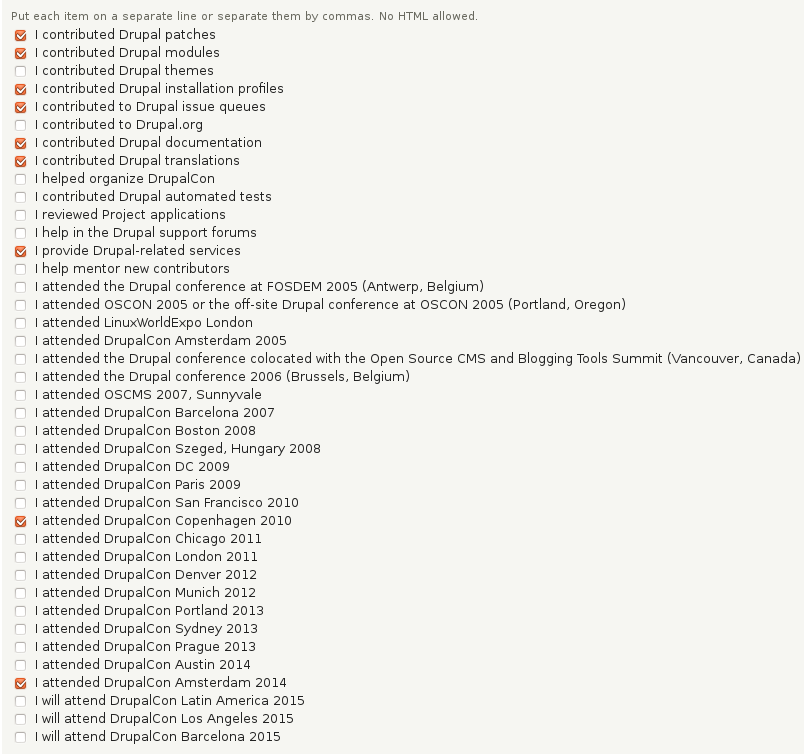
\includegraphics[scale=0.45]{img/profiles/list_contributions.png}
        \caption[List of contribution activities in the ``Drupal" section of my profile]%
        {List of contribution activities in the ``Drupal" section of my profile. Retrieved \nth{22} October 2014, from \url{https://www.drupal.org/user/740628/edit/Drupal} (not available unless logged in), under a CC BY-SA 2.0 license.}
        \label{profiles_list_contributions}
    \end{figure}

    \begin{figure}[H]
        \centering
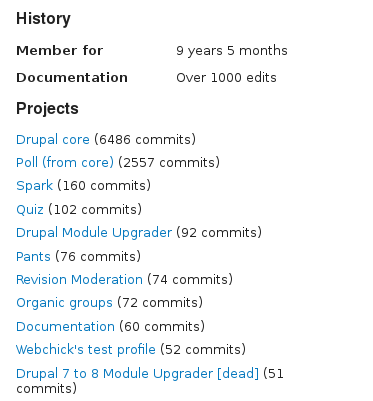
\includegraphics[scale=0.45]{img/profiles/code_documentation.png}
        \caption[Example of quantified contributions related to source code and documentation]%
        {Example of quantified contributions to source code and documentation. Retrieved \nth{5} November 2014, from \url{https://www.drupal.org/u/webchick}, under a CC BY-SA 2.0 license.}
        \label{profiles_code_documentation}
    \end{figure}

    \begin{figure}[H]
        \centering
        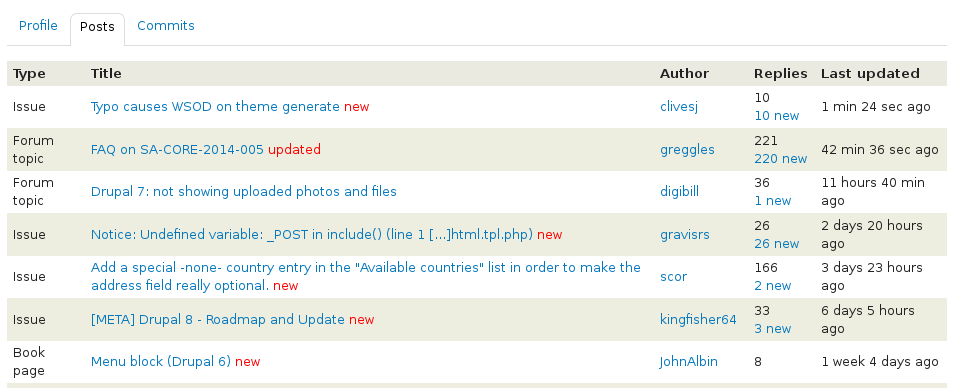
\includegraphics[scale=0.45]{img/profiles/posts.png}
        \caption[Example of list of posts listed in the tab ``Posts" of the user profile]%
        {Example of list of posts listed in the tab ``Posts" of the user profile. Retrieved \nth{5} November 2014, from \url{https://www.drupal.org/user/338895/track}, under a CC BY-SA 2.0 license.}
        \label{profiles_posts}
    \end{figure}

    \begin{figure}[H]
        \centering
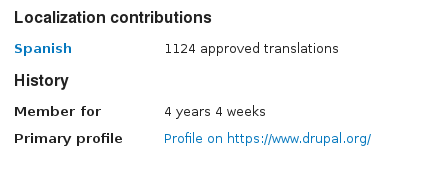
\includegraphics[scale=0.5]{img/profiles/translations_profile.png}
        \caption[Example of quantified contributions related to translation activities]%
        {Example of quantified contributions related to translation activities. Retrieved \nth{5} November 2014, from \url{https://localize.drupal.org/user/311048}, under a CC BY-SA 2.0 license.}
        \label{profiles_translations}
    \end{figure}

    \begin{figure}[H]
        \centering

\includegraphics[scale=0.5]{img/profiles/profiles_bio2.png}
        \caption[Example of use of the open field ``Bio" to display contributions about evangelisation activities]%
        {Example of use of the open field ``Bio" to display contributions about evangelisation activities. Retrieved \nth{5} November 2014, from \url{https://www.drupal.org/u/rob_feature}, under a CC BY-SA 2.0 license.}
        \label{profiles_bio2}
    \end{figure}

    \begin{figure}[H]
        \centering

\includegraphics[scale=0.5]{img/profiles/profiles_mentors.png}
        \caption[Example of the use of the field ``Mentors" to acknowledge mentorship contributions in a peer-to-peer way]%
        {Example of the use of the field ``Mentors", to acknowledge mentorship contributions in a peer-to-peer way. Retrieved \nth{5} November 2014, from \url{https://www.drupal.org/u/lewisnyman}, under a CC BY-SA 2.0 license.}
        \label{profiles_mentors}
    \end{figure}

    \begin{figure}[H]
        \centering
        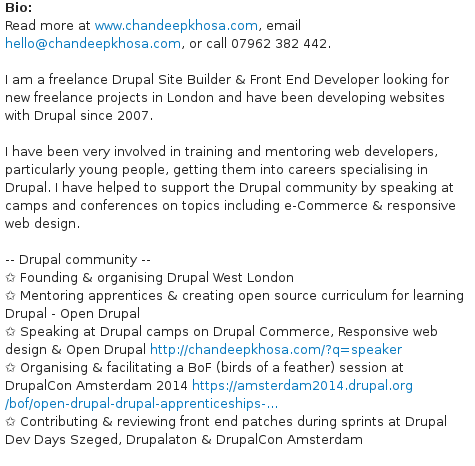
\includegraphics[scale=0.5]{img/profiles/profiles_bio.png}
        \caption[Example of the use of the open field ``Bio" to display contributions about mentoring and face-to-face events activities]%
        {Example of the use of the open field ``Bio" to display contributions about mentoring and face-to-face events activities. Retrieved \nth{5} November 2014, from \url{https://www.drupal.org/u/chandeepkhosa}, under a CC BY-SA 2.0 license.}
        \label{profiles_bio}
    \end{figure}

    \begin{figure}[H]
        \centering
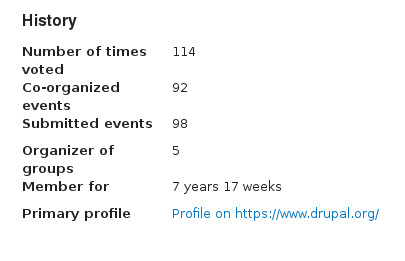
\includegraphics[scale=0.5]{img/profiles/groups_drupal_org.png}
        \caption[Example of quantified contributions related to online community management activities]%
        {Example of quantified contributions related to online community management activities. Retrieved \nth{5} November 2014, from \url{https://groups.drupal.org/user/8713}, under a CC BY-SA 2.0 license.}
        \label{profiles_groups}
    \end{figure}

    \begin{figure}[H]
        \centering
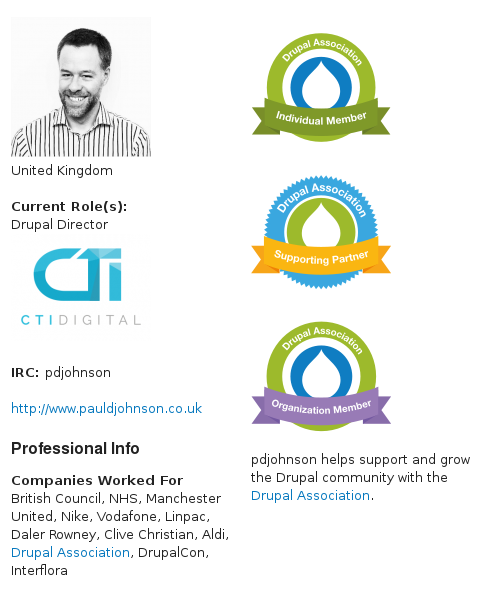
\includegraphics[scale=0.45]{img/profiles/badgets_and_pic.png}
        \caption[Example of badges provided by the Drupal Association]%
        {Example of badges provided by the Drupal Association. Retrieved \nth{5} November 2014, from \url{https://www.drupal.org/u/pdjohnson}, under a CC BY-SA 2.0 license.}
        \label{profiles_badgets}
    \end{figure}

    %% END LIST OF FIGURES

The analysis, summarised in the previous tables, shows an uneven representation of contribution activities in user profiles at Drupal.org. Overall, this affects the activities within the ``community-oriented" category (G\textunderscript{2}) far more than those in the ``object-oriented" category (G\textunderscript{1}). The exceptions for G\textunderscript{1} are ``design" (SG\textunderscript{1.4}) and ``\textit{custom} projects" (SG\textunderscript{1.1.3}). In the case of the former, however, it was found that Drupalistas use generic open text fields to overcome these limitations. For the case of the latter, the lack of representation can be explained on the basis of the lack of perceived value of code outside of the main platform of collaboration, since it is not subject to peer-reviewing processes, as will be more extensively discussed in chapter \ref{sec:custom-to-contrib}.

Nevertheless, the most severe lack of representation is found in contribution activities related to the organisation of and participation in local events (SG\textunderscript{2.5.1}), \textit{DrupalCamps} and role-oriented events (SG\textunderscript{2.5.2}). Furthermore, in these cases a prominent use of open text fields by Drupalistas was found,  as illustrated in figure \ref{profiles_bio}. This can be explained as a way in which Drupalistas try to overcome these limitations, providing an indicator of the unfulfilled need to have these traditionally less visible contributions publicly acknowledged.

This analysis of user profiles provides, firstly, a descriptive account of how the contribution activities identified in the previous subsection are represented in the different user profiles on the main collaboration platform; but most importantly the analysis provides empirical evidence of the uneven representation of certain contribution activities, affecting especially those identified as ``community-oriented".

\section{``Come for the software, stay for the community": the role of affective labour in the Drupal community}
\label{subsec:insights:affective-labour}

A strong sense of community is often mentioned by Drupalistas. This sense of community is even present in Drupal's main motto: ``Come for the software, stay for the community\footnote{See \url{https://www.drupal.org/}, accessed on \nth{30} April 2014.}". However, the mechanisms that enable the creation of this sense of community are less clear.

In this subsection, the focus is placed on the role that the organisation of and participation in face-to-face events plays to create this sense of community, since they emerged as the clearest example of this in the analysis. This is conceptualised drawing on the concept of affective labour \parencite{hardt1999affective} as outcomes of these activities. By affecting the emotional experiences of Drupalistas, in a variety of ways depending on their experience,  these contribution activities play a relevant role in the sustainability of the community, although they are less visible in terms of representation. Many outcomes that can be interpreted as affective labour from these contribution activities were found. However, a significant difference in perception was found depending on the degree of experience of the Drupalista. For example, participation in face-to-face events was commonly described by new members as a way to humanise the community. Drupal is regarded not just as ``a piece of software", but rather a community in which Drupalistas become commoners through ``commoning" \parencite{linebaugh2008magna}. The following excerpt from I\textunderscript{2}, while reflecting on how attendance at local meetings changed his emotional experiences, illustrates this:

\begin{quotation}
    ``[...] indeed, the fact of attending these meetups was really good. Because you realise there are people behind the source code, right? There are people behind the modules. And you meet people that can tell you a kind of personal story. [...] And then, it stops being something anonymous, it becomes something yours."

\begin{flushright}\footnotesize{Drupal developer and devop, M, 1 year. Original reply in Spanish.}\end{flushright}
\end{quotation}

Another common outcome of participation for new members was help with avoiding barriers, and increasing the will to contribute. The following excerpt from a new member after attending a \textit{DrupalCamp} for the first time illustrates this type of outcome:

\begin{figure}[H]
    \centering
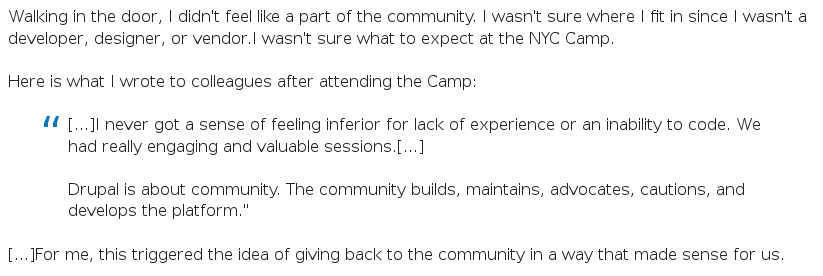
\includegraphics[scale=0.51]{img/quotes_replacement/quote_olympus.png}
    \caption[Excerpt from the article ``Guest Post: Why Olympus Gives Back to Drupal"]{Drupal project manager, M, 1 year. Excerpt from the article ``Guest Post: Why Olympus Gives Back to Drupal". Retrieved \nth{22} May 2014, from \url{https://assoc.drupal.org/content/guest-post-why-olympus-gives-back-drupal}. Drupal Association.}
    \label{quote_olympus}
\end{figure}

As the engagement with the commons increases, affectionate relationships develop, to the point of friendship in some cases. A veteran Drupalista, I\textunderscript{3}, described the role that face-to-face ``meetups" play in forming friendships:

\begin{quotation}
    ``[...] friendships are developed, and seeing people in-person helps a lot. I believe the idea of having face-to-face meetups and getting to know each other in-person is essential. [...] In the IRC [Internet Relay Chat] you will talk about certain things, but after a day cycling 50 or 60 kilometres [referring to the `Tour de Drupal\footnote{See footnote \ref{footnote-drupal}.}'], when you go to have dinner with that person, probably the conversation topics might be different... or the same. But there will be more interaction for sure, and a greater friendship [...]"

\begin{flushright}\footnotesize{Drupal developer, M, 7 years. Original reply in Spanish.}\end{flushright}
\end{quotation}

These relationships remain afterwards, even if the Drupalistas are in different locations or are unable to see each other often. When asked about the establishment of relationships in the Drupal community, I\textunderscript{4} explained:

\begin{quotation}
    ``[...] I've got really good friendships with people. And I've got a lot of people I'm kind of actively in touch with all the time. But there's also this thing I feel like... I've got friends who are, you know, old friends I've known in the Drupal community, that I haven't seen for a long time. [...] But if they were just to pop up on my doorstep, it would just be like carrying on from where we left off. [...] You know, it's like... we are such close friends that, we don't need to continue to keep in touch."

\begin{flushright}\footnotesize{Drupal themer and developer, M, 11 years.}\end{flushright}
\end{quotation}

Furthermore, local activities become more critical as the community grows, allowing the sense of community to scale up. I\textunderscript{4} expressed how, since the Drupal community has been constantly growing, the emergence of more but smaller local communities enables the maintenance of this sense of community:

\begin{quotation}
    ``Because the community is growing, then you have less of a sense of community. But I think the solution to that is to have smaller local communities. So, you know, as the worldwide community grows, then you start finding, like whereas before it might have been 50 people worldwide, now you have like 50 people in your part of London, or wherever."

\begin{flushright}\footnotesize{Drupal themer and developer, M, 11 years.}\end{flushright}
\end{quotation}

This subsection has focussed on the relevance of face-to-face events, as an illustration of the existence and relevance of affective labour in the Drupal community. These events emerged as the most prominent source of affective labour during the study. Hence, it is not only that ``community-oriented" activities such as these are understood as a type of contribution, as shown in subsection \ref{subsec:insights:contrib-beyond-source-code}; nor is it only that they are unequally represented in the main collaboration platform, as presented in subsection \ref{subsec:insights:representation}; but they play a key role in the sustainability of the community, as shown in this subsection. They provide  emotional experiences for their participants and help to foster collaboration.

\section{Discussion}
\label{sec:discussion}

Previous research on FLOSS communities has highlighted the importance of face-to-face events in these communities. For instance, in her ethnographic study of hacker culture using the FLOSS Debian community as a case study, Coleman described the relationship between the conference (DebConfs) and the public as having ``affective, moral, economic, and political dimensions" \parencite[59]{coleman2013coding}.  She described the importance of these conferences to foster collaboration. They created the basis for social solidarity and for the establishment and sustainability of relationships: ``[...] people embark on decisions and actions they probably would not have considered otherwise. Some hackers decide to formally apply to become a Debian developer, while longtime developers  decide not to quit the project" \parencite[57]{coleman2013coding}. This study provides additional evidence of the importance of such activities, but extends this by arguing how they are understood as relevant contributions.

A similar perspective is shared in \citeauthor{nordinmotivation2014}'s (\citeyear{nordinmotivation2014}) study, in the field of information design, on the barriers experienced by Drupal contributors, which was carried out at almost the same time as that presented in this chapter. Although Nordin's study was focussed on providing a set of guidelines to improve Drupal.org in order to overcome these barriers, she also reconsidered the notion of contribution concluding that ``metrics such as code commits used to gauge contribution by Open Source literature and by Drupal.org itself paint an incomplete picture of the types of contributions that actually happen in the Drupal project" \parencite[][43]{nordinmotivation2014}. The findings presented in this study provide further evidence of the role which less visible contributions, such as the organisation of and participation in face-to-face local events, play in transforming emotional experiences, as well as helping to scale up the sense of community, aspects which were not addressed by \textcite[][28-30]{nordinmotivation2014}.

Furthermore, by drawing on the concept of ``affective labour", this study connects the findings with the larger literature on the commons. Participation in the Drupal community ``transforms the local subjectivities" of Drupalistas, in a way reminiscent of \textcite{Singh2013}, in her research on community-based forests in India. By looking at an extreme ``code-centric" case study, this research provides additional empirical evidence of the importance of affective labour in CBPP communities, which was argued by \textcite{Bollier2014} to be its ``lifeblood".

The lack of representation of ``community-oriented" activities cannot be understood as due solely to socio-cultural reasons. The ``code-centric" character of the community offers only a partial explanation. Technical limitations also have a major impact. For example, while certain activities are easily quantifiable (e.g. the number of commits of source code, or the number of editions of wiki pages), others are more difficult to  quantify or represent in concise, useful ways. In some cases, although  indicators are available, the information is beyond the scope of, and therefore not reflected in, the main collaboration platform. For example, external platforms such as Meetup.com, commonly employed for the organisation of local events, provide an account of the number of events attended and organised by a certain user. Nevertheless, this information is stored in proprietary third-party platforms and therefore absent from Drupal.org.

However, the main limitation lies in the difficulty to provide indicators to measure and aggregate the value of some types of contribution, or even distribute it beyond the CBPP community itself; an issue that is under exploration by researchers \parencite[e.g.][]{de39measuring} as well as CBPP communities \parencite[e.g.][]{ova-value:Online} themselves. The Drupal community is also attempting to find suitable indicators. For example, there is an ongoing initiative\footnote{See \url{https://www.drupal.org/node/2305759}, accessed on \nth{15} September 2014.} to improve how activities are represented in user profiles at Drupal.org, to ``[...] go beyond code creation activity and into more community-oriented contribution stuff, since that's also a huge part of what makes Drupal healthy.", and some of the elements, such as the peer-to-peer mentorship references illustrated in figure \ref{profiles_mentors}, indicate the will to follow that direction\footnote{Indeed, a new version of user profiles (see \url{https://www.drupal.org/user/}, accessed on \nth{24} February 2015) was released months after this study concluded, confirming the will to advance in that direction. For example, the mentorship relationships depicted in figure \ref{profiles_mentors} are now highlighted by including their pictures, and they are also quantified inversely, by listing the number of users who list that profile as a mentor.}.

Overall, this issue should be understood within the wider context of CBPP, and the need to enhance and expand the conceptualisation and measurement of value in these communities, as well as the incorporation of indicators of such contribution into the socio-technical systems employed to support their organisation. This is an aspect that becomes especially relevant in large and global communities as they scale up since, due to their growth and their global character, the generation of perceptions between unknown members becomes more frequent in these communities, and the role of the platforms employed to support their self-organisation becomes more relevant.

\section{Conclusion}

By studying an extreme ``code-centric" case study, the findings presented in this chapter expose the need to broaden our understanding of contribution activities in FLOSS communities beyond the most easily quantifiable and ``object-oriented". The ethnographic approach taken showed how certain activities, whose focus is directed towards the community, are indeed understood as contributions. These activities foster collaboration, as well as affecting the creation or modification of emotional experiences, varying according to the degree of experience of the participants.

Most of these contributions are poorly represented in the main collaboration platform as compared to ``object-oriented" ones. This unequal representation was found at an ``official" level, such as in the main sections of the platform dedicated to contribution, as well as at an individual level, such as in the study of user profiles. This disjunction between the relevance and lack of visibility of this type of contribution casts doubt on the ``object-centric" myth illustrated in the motto ``Talk is silver, code is gold", which has been traditionally present in FLOSS communities.

These findings extend previous studies on FLOSS to connect it to the wider area of CBPP, drawing on the concept of affective labour. Through  participation in ``commoning" processes, the subjectivities of  participants are transformed.

Having explored the notion of contribution in the Drupal community, the conceptual underpinnings necessary to further explore the study of self-organisation in the Drupal community by focussing on contribution activities are laid out. Concretely, chapters \ref{sec:custom-to-contrib} and \ref{chapter:core-system} will address the study of the development of projects, while chapters \ref{mostly-offline-local:chapter} and \ref{mostly-offline-cons:chapter}, the organisation of events.